%%%%%%% SOFTWARE NODES %%%%%%
%\addcontentsline{toc}{subsection}{Software nodes}
\subsection{Nodes}
\label{nodes}


The processing needed to provide all the functionality is divided in nodes. Here they are presented, ordered using the data work-flow, beginning the ones using the raw input data to the system and finishing with the ones that deliver the output of the system. 
\\


\subsubsection{\large Converter}\\
		\label{converter}

	This node is the first step of the code. It transforms the input data from the pi\_tracker package into the custom message used within the software. The information provided by that third-party code contains the position in the space of each joint of the body. The converter node takes only both hand's position. 
	\\

	It use case diagram of the node can be seen in the diagram below: 

	\begin{figure}[H]
		\centering
	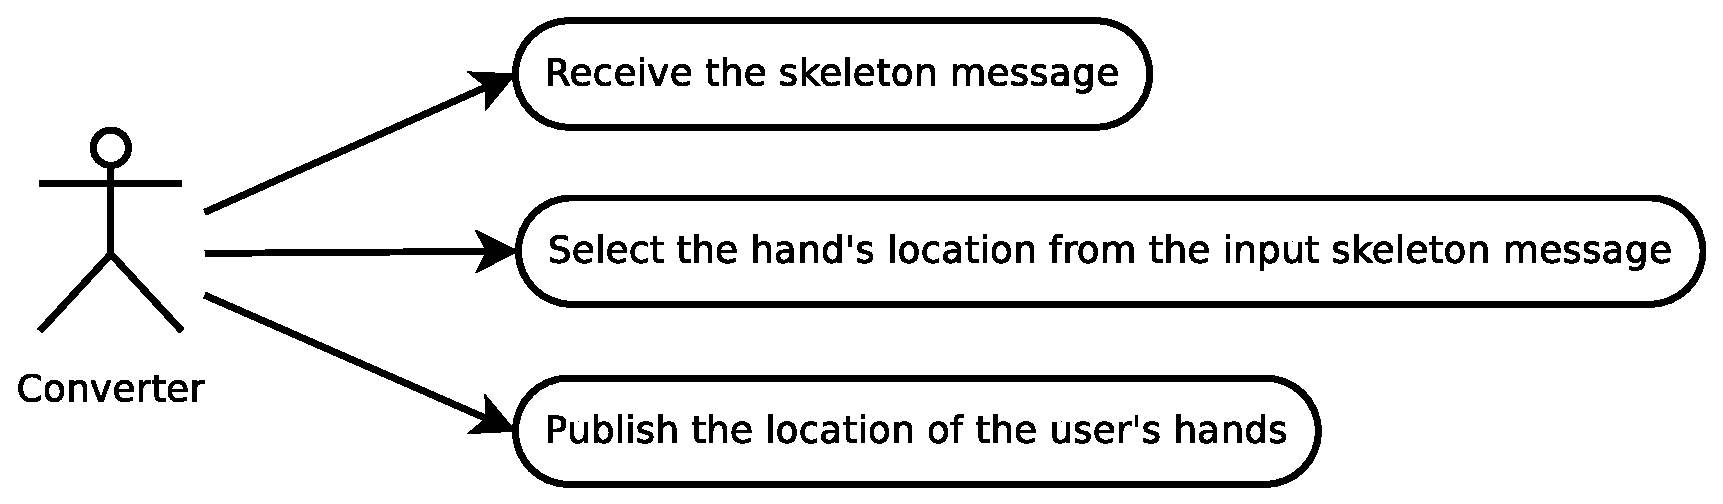
\includegraphics[scale=0.4]{img/diagrams/uc_converter.eps}
		\caption[Use case diagram converter node]{Use Case diagram of the converter node}
		
	\end{figure}

	
\subsubsection{ROI Segmenter 3D}\\
	\label{roi_segmenter_3d}

	The input of this node is the raw 3D information from the sensor and the hand's locations from the third-party package pi\_tracker, as well as the hand in which the user is holding the object. The node segments a prism from the original point cloud around the selected hand's center. The prism vertices coordinates are transformed from world coordinates to pixels. That information is the output of the node, together with the segmented point cloud. 

	\begin{figure}[H]
		\centering
	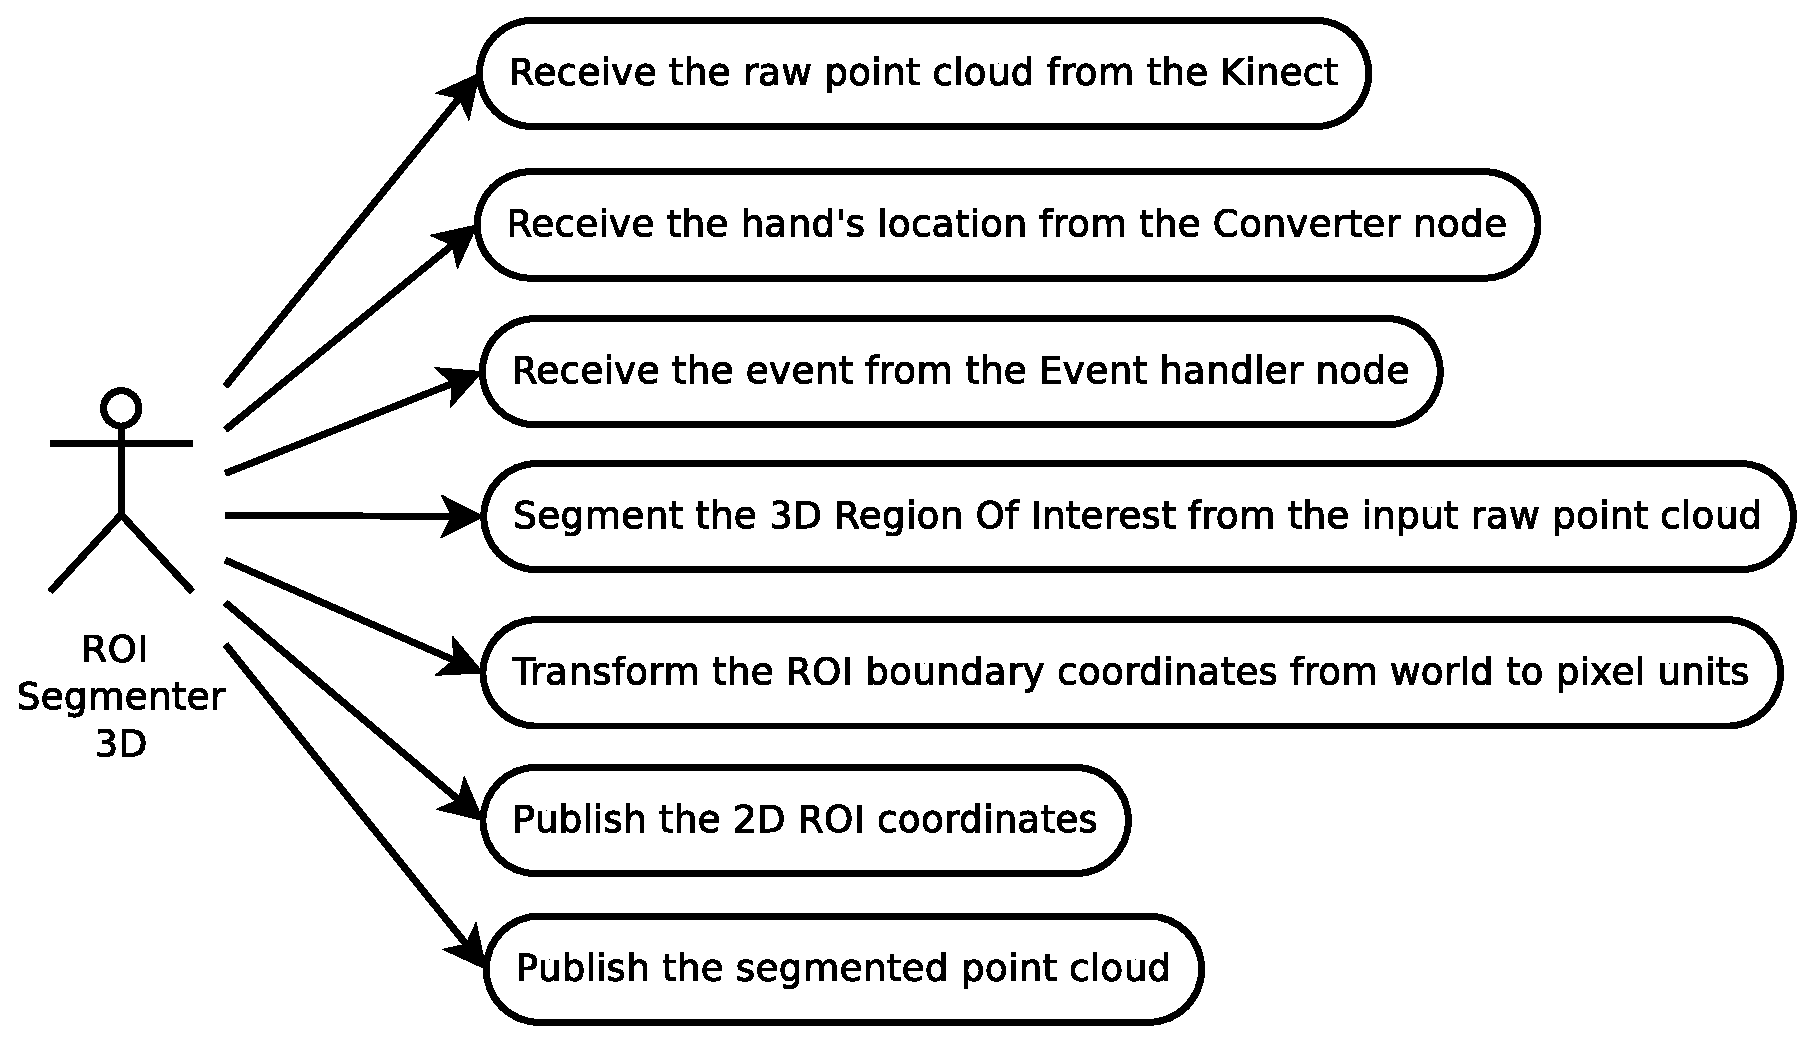
\includegraphics[scale=0.4]{img/diagrams/uc_roi_segmenter_3d.eps}
		\caption[Use case diagram ROI segmenter 3D node]{Use Case diagram of the ROI segmenter 3D node}
		
	\end{figure}
 
\subsubsection{ROI Segmenter 2D}\\
	\label{roi_segmenter_2d}
	The present node takes as the input the raw 2D information from the RGB-D sensor and the hand's locations in pixels returned from the ROI segmenter 3D node. Then, it extracts the ROI (Region Of Interest) taking a square section around the center of the hand. The size of that figure is fixed for simplicity. Since due to the RGB-D sensor's current resolutions the user must remain at a fixed distance from the sensor, the difference in the scale due to the distance is negligible and hence the size can be fixed. 
	\\

	In the following image the use case diagram of the node can be observed.
	\begin{figure}[H]
		\centering
			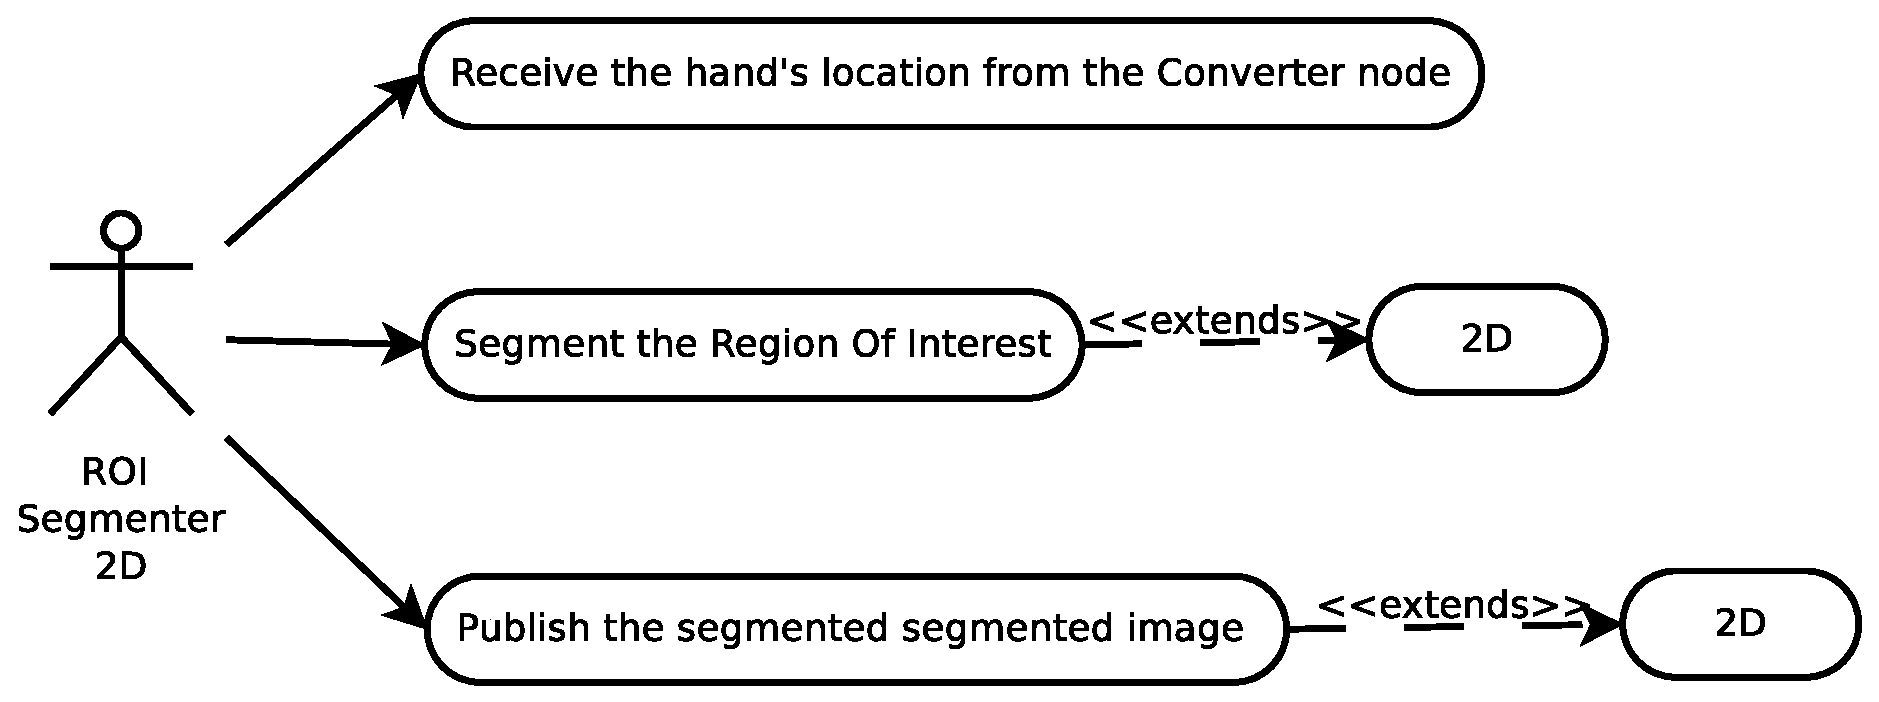
\includegraphics[scale=0.4]{img/diagrams/uc_roi_segmenter_2d.eps}
			\caption[Use case diagram ROI segmenter 2D node]{Use Case diagram of the ROI segmenter 2D node}
		
	\end{figure}


\subsubsection{Feature Extractor 2D}\\
	This node takes as an input the segmented 2D ROI from the previous nodes and extracts the features. The output of the system is a matrix with the descriptors values. The method used in order to compute the features was presented previously in the section  \ref{features}.

	\\

	The following figure represents the use case diagram of this node. 
	\begin{figure}[H]
		\centering
			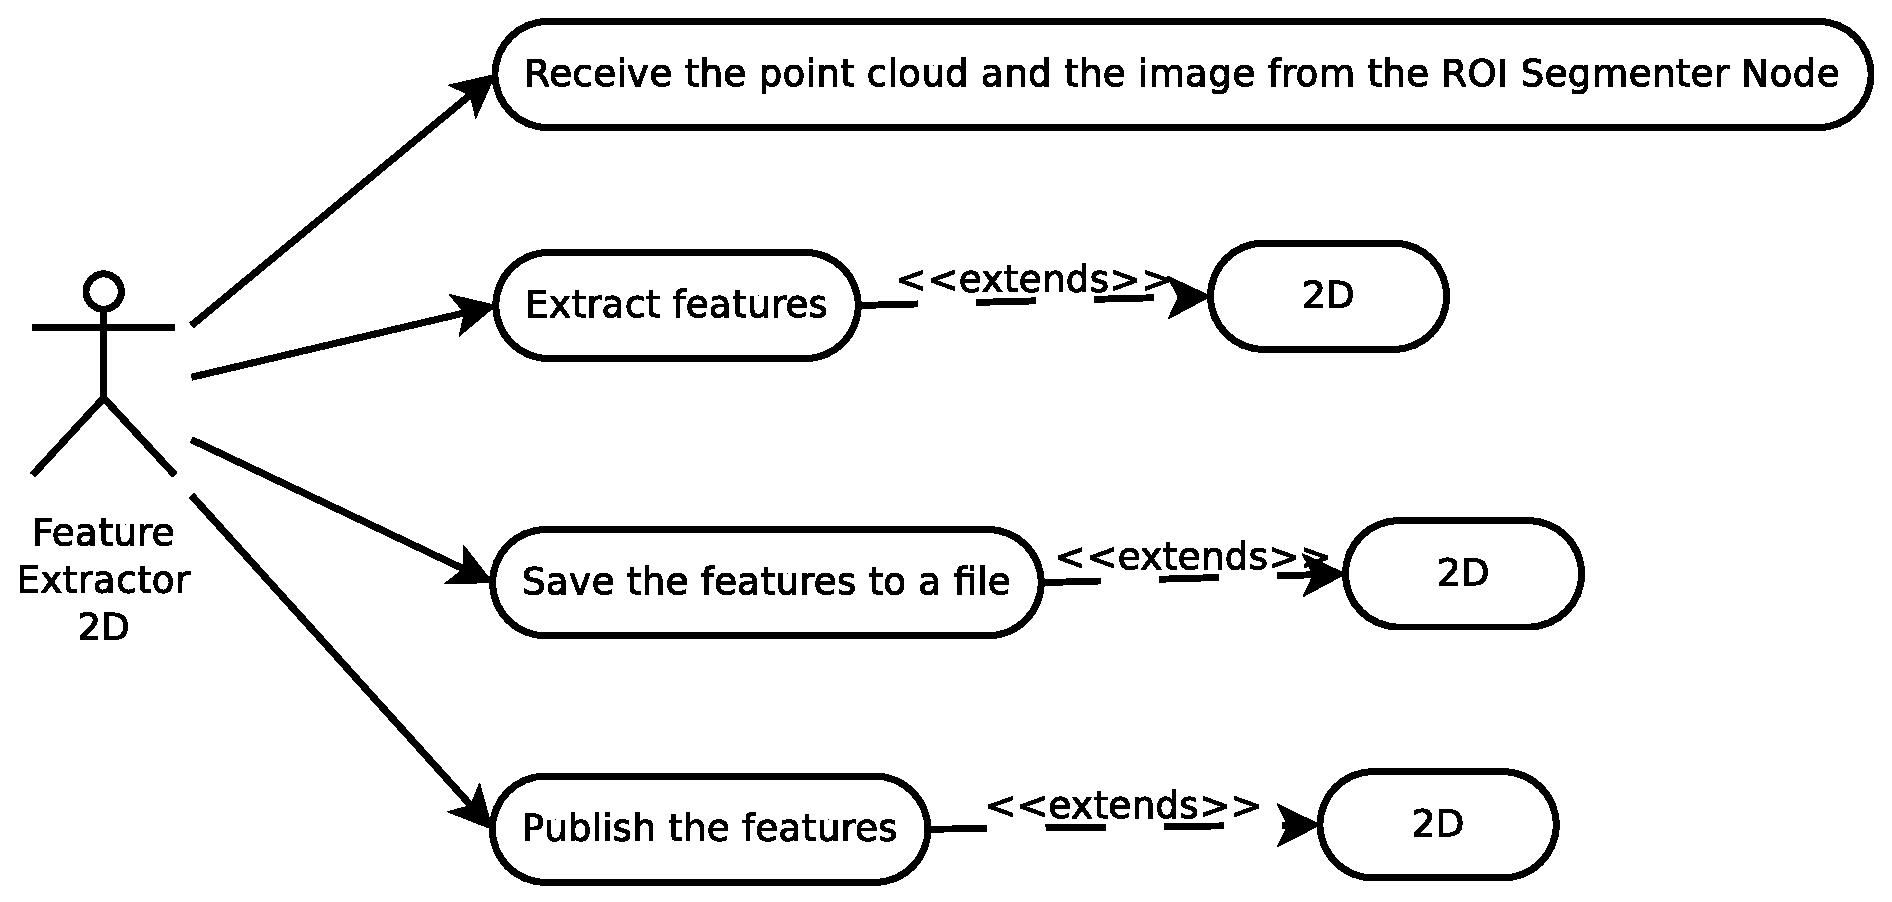
\includegraphics[scale=0.4]{img/diagrams/uc_feature_extractor_2d.eps}
			\caption[Use case diagram Feature Extractor 2D node]{Use Case diagram of the Feature Extractor 2D node}
		
	\end{figure}

\subsubsection{Feature Extractor 3D}\\
	The input of this node is the segmented point cloud from the ROI Segmenter 3D node. The descriptors are extracted from this information and are published in the output topic. 
	\\

	The picture below shows the use case diagram of the node. 

	\begin{figure}[H]
		\centering
			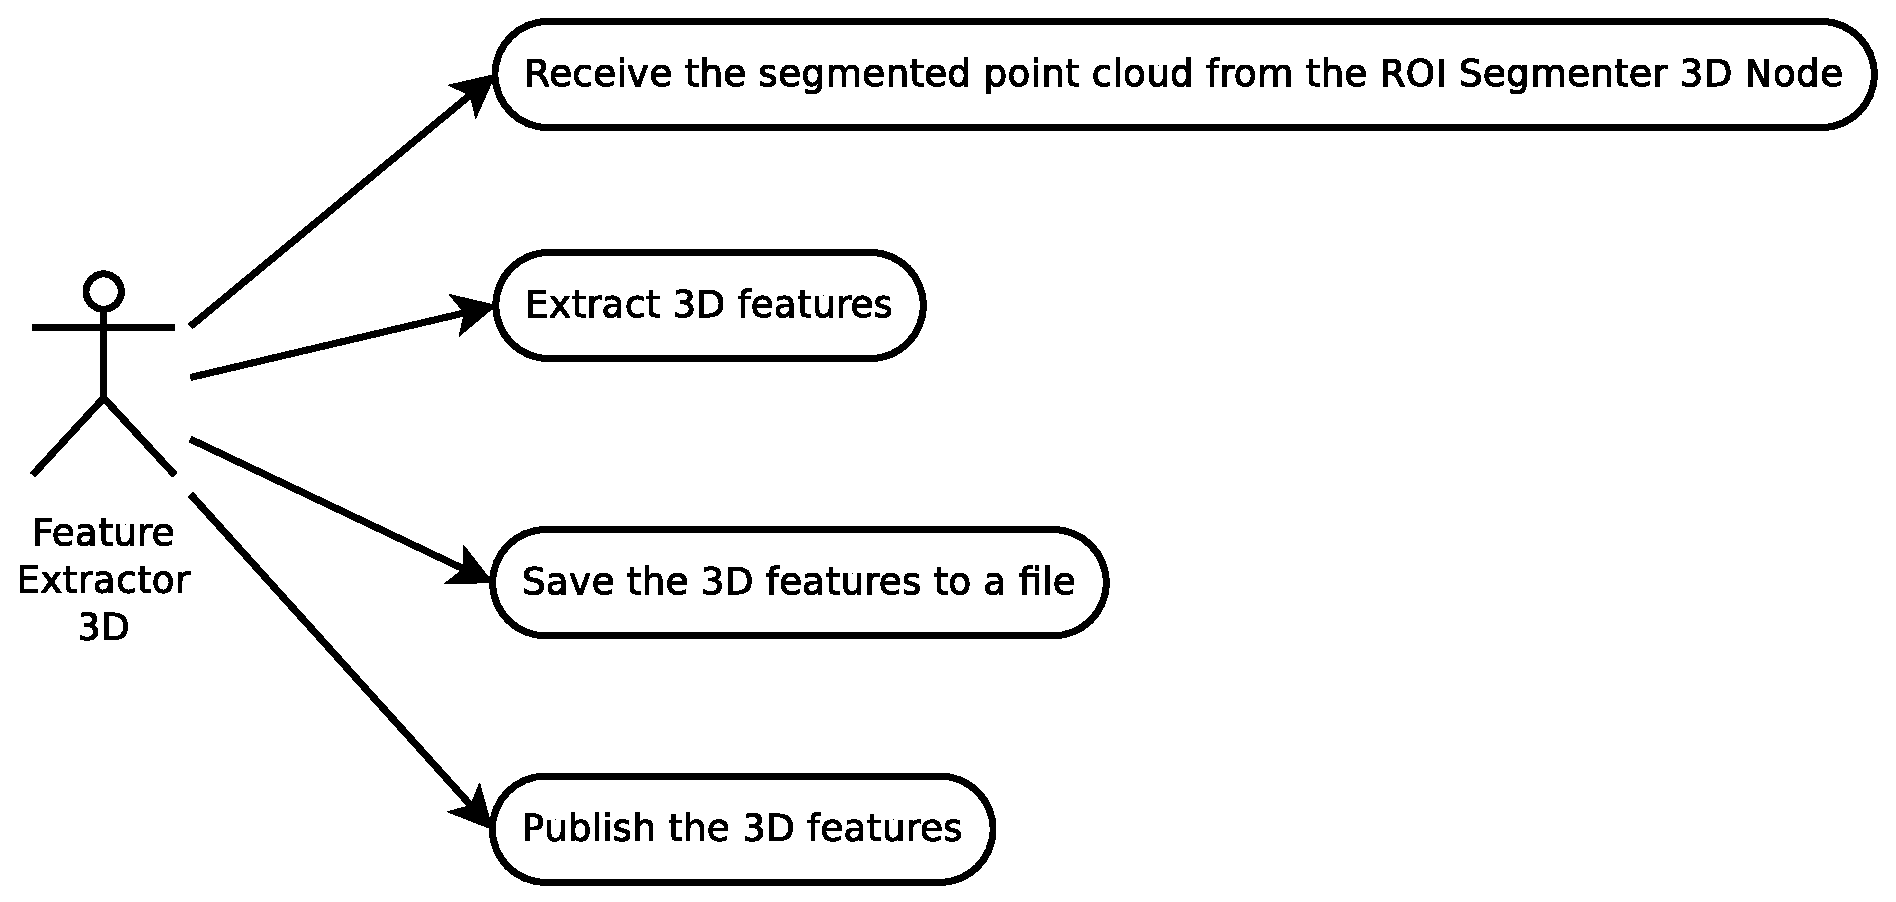
\includegraphics[scale=0.4]{img/diagrams/uc_feature_extractor_3d.eps}
			\caption[Use case diagram Feature Extractor 3D node]{Use Case diagram of the Feature Extractor 3D node}
		
	\end{figure}

\subsubsection{Event Handler}\\

	This is the node responsible of detecting the different event that can appear in the software usage. As it was previously stated, in order to interact with the software some gestures were defined. This is the module that detects those gestures and switches accordingly to the corresponding event. 
	\\

	The input of the system is the skeleton message that is obtained from the third-party package pi\_tracker. This message contains the information of all the joints of the user. The information is screened to detect the height at which each hand is located. The one that is the highest is the one being used in the software. Afterwards, the distance between the body and the chosen hand is computed. When that distance is similar to the distance of the user's arm, the event triggered is "learn". If, otherwise, the hand is located close to the body, the event that is published to the output topic is "recognize". 
	\\

	The distance that triggers the modes is proportional to the distance between the user and the RGB-D sensor in order to obtain a range of use of the software higher. 
	\begin{figure}[H]
		\centering
			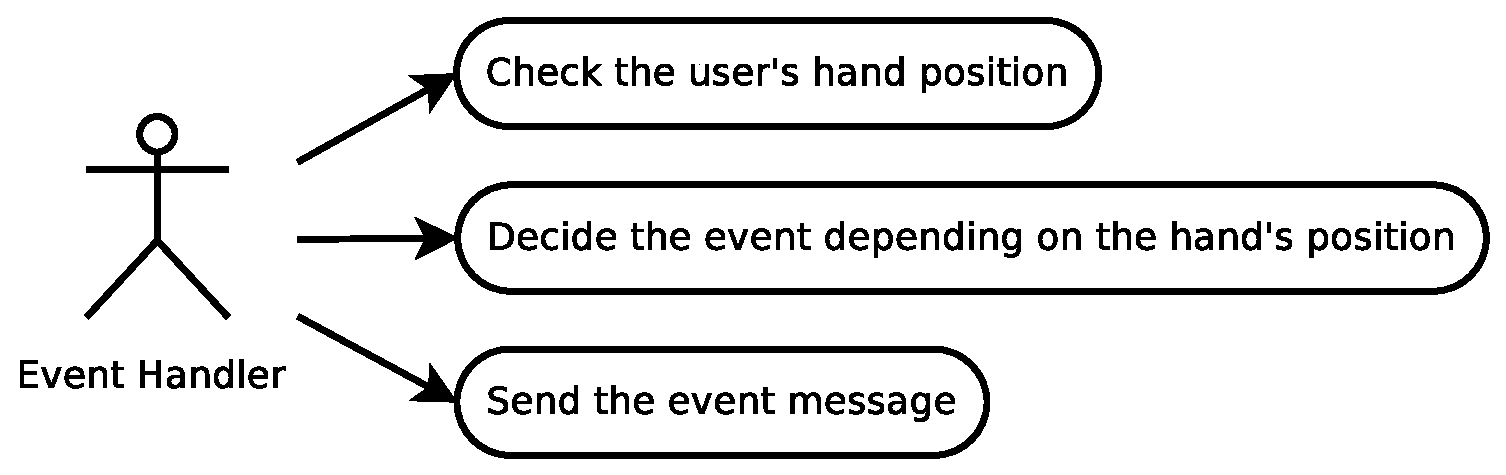
\includegraphics[scale=0.4]{img/diagrams/uc_event_handler.eps}
			\caption[Use case diagram Event Handler node]{Use Case diagram of the Event Handler node}
		
	\end{figure}

\subsubsection{Learner Recognizer}\\
\label{learner_recognizer}

	This node is the one that implements the state machine depending on the events recognized by the previous node. If the event received is "learn", the learning sequence starts. If the event is "recognize", the recognize sequence is triggered. 
	\\

	The learn sequence consists on obtaining and storing the features both 2D and 3D and waiting a second allowing the user to move the object to capture a new view of it. 
	\\

	The recognition sequence compares the newly obtained features both 2D and 3D with the ones that are stored in the dataset. Afterwards, a decision algorithm is followed and the result of the recognition published in the output topic. This is the output of the whole software. 

	\begin{figure}[H]
		\centering
			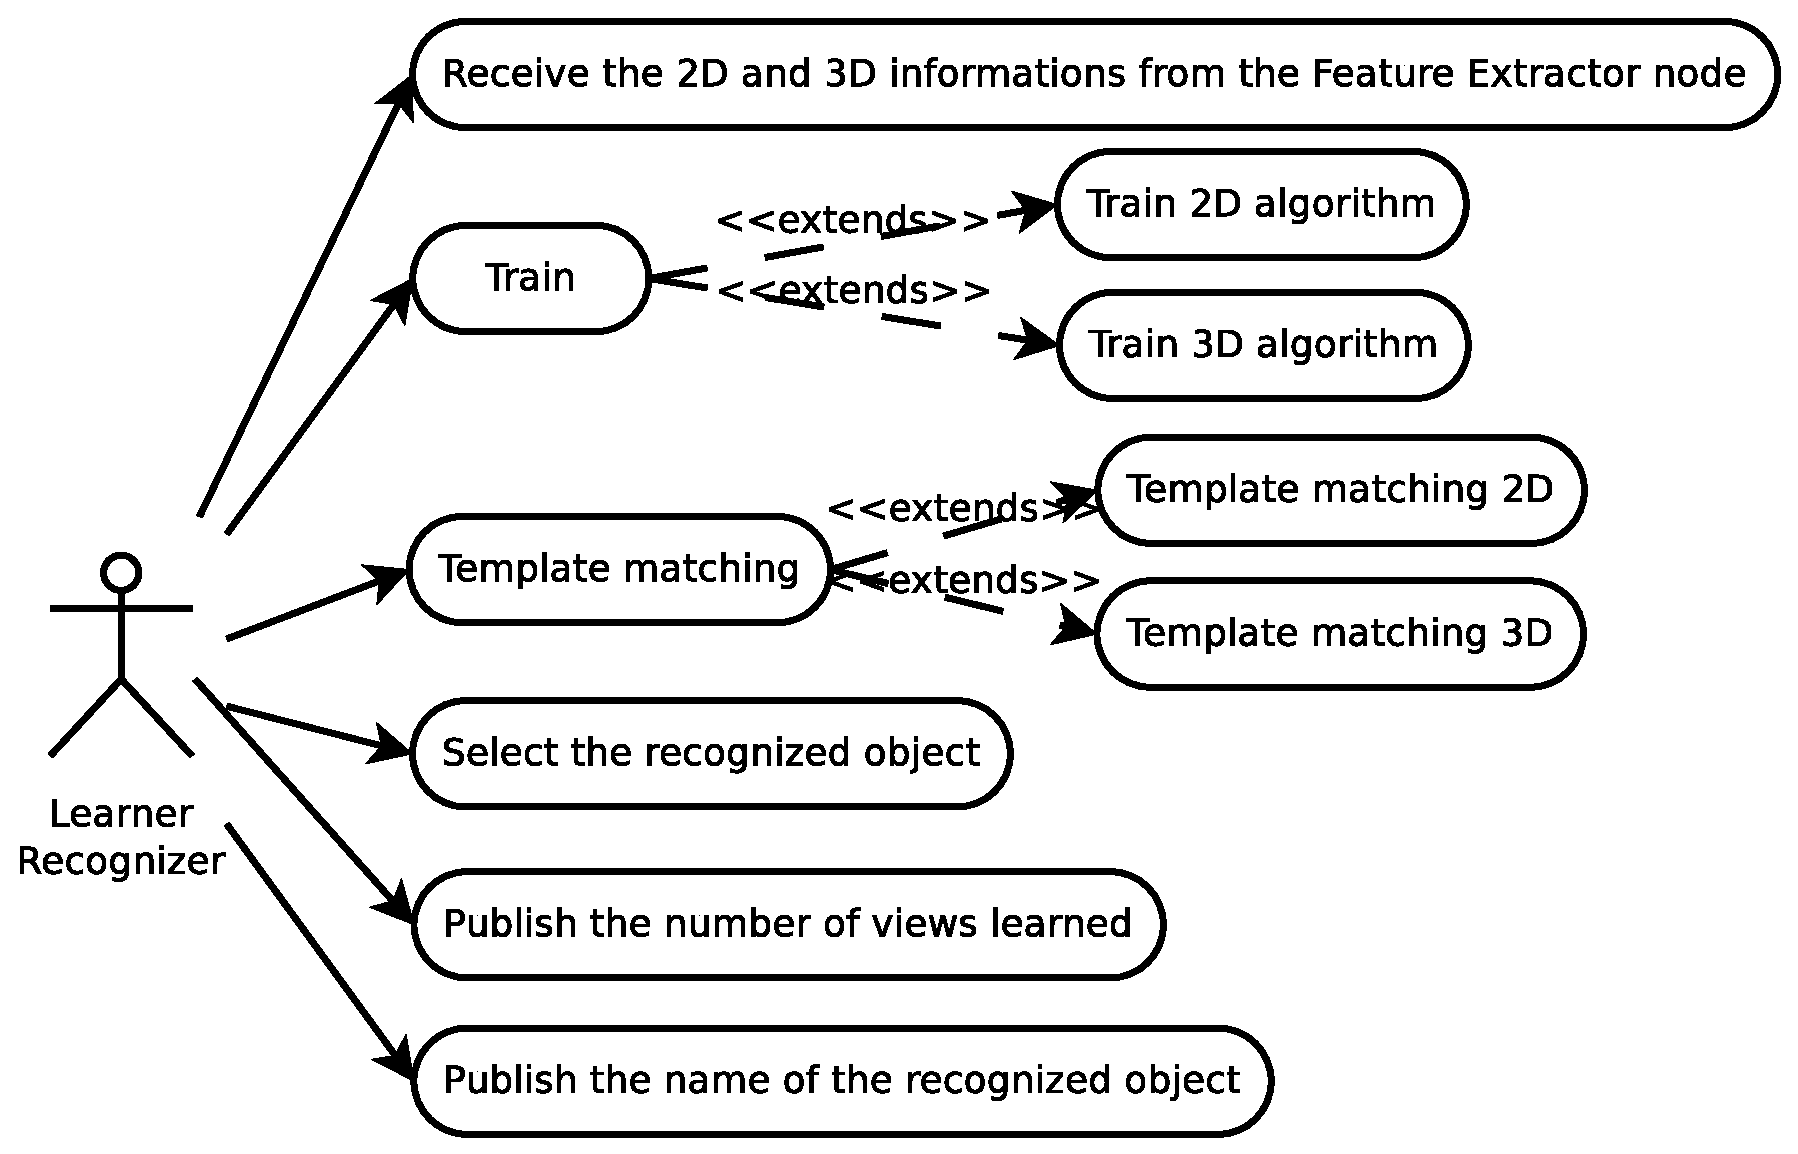
\includegraphics[scale=0.4]{img/diagrams/uc_learner_recognizer.eps}
			\caption[Use case diagram Learner Recognizer node]{Use Case diagram of the Learner Recognizer node}
		
	\end{figure}



